
\documentclass[addpoints]{exam}
\usepackage{url}
\usepackage{amsmath,amsthm,amssymb,enumitem}
\usepackage{graphicx}
\usepackage{algorithm}
\usepackage{algpseudocode}
\usepackage[dvipsnames]{xcolor}
\usepackage[top=1.5cm, bottom=2.5cm, left=2cm, right=2cm]{geometry}
%\input myfonts

%\def\mysolution#1{#1} % Uncomment this to reveal answers
\def\mysolution#1{}    % Uncomment this to hide answers 

\newtheorem*{claim}{Claim}
\title{CS 6150 - Fall 2025 - HW1 \\ Data structures, Divide and conquer, Dynamic programming}
\date{Submission date: Friday, Sep 26, 2025 (11:59 PM)}
\begin{document}
\maketitle
\begin{center}
\fbox{\fbox{\parbox{5.5in}{\centering 
This assignment has \numquestions\ questions, for a total of \numpoints\
points. You will still be graded out of 100, and any points you earn above 100 will count as bonus and can compensate for a low score on other homeworks.
Unless otherwise specified, complete and well-reasoned formal arguments are expected in all answers. }}}
\end{center}

\qformat{Question \thequestion: \thequestiontitle\dotfill \textbf{[\totalpoints]}}
\pointname{}
\bonuspointname{}
\pointformat{[\bfseries\thepoints]}

\begin{center}
  \gradetable
\end{center}
\newpage
\begin{questions}
\titledquestion{Prefix trees / tries}
Prefix trees can be used as a ``poor man's binary search tree''. Let us see the sense in which this is true. Suppose we have a set of $N$ integers all in the range $[0, 2^k - 1]$ for some constant $k$. If we treat them as strings in base $2^d$ (assume $d$ divides $k$) and use a trie data structure to store them:
 
\begin{parts}
\part[4] How many characters (at most) are needed to represent any integer in the given range in base 2 (i.e. binary) and in base $2^d$?

\textbf{We know that with k bits we can represent $2^k$ different numbers in binary. Because of this fact we know that to represent any integer in the given range in base $2$ we would need at most $k$ bits.}

\textbf{Figuring out how many characters are needed in base $2^d$ is a little more tricky. The technique to do this is to set your $k$ to something fixed like $4$. Then check and see how many characters are needed to represent the largest number in the divisible values of d. In this example we would check how many characters are needed to represent $15$ with $d=1,2,4$. From this the patern emerges that you need $\frac{k}{d}$ characters to represent all possible numbers in the given range. See 'Problem 1a.png' for detailed work.}

\mysolution{
\input{Sol-1a}
}

\part[4] What is the depth of the trie constructed as described above?
\textbf{The maxium depth of the trie constructed as above would simply be the number of characters needed to represent all numbers in the range. This would also be $\frac{k}{d}$}

\mysolution{
\input{Sol-1b}
}
\part[2] How long is the query time and insertion time in this trie? (Assume the integer is already converted to base $2^d$.)

\textbf{Both the insertion time and the query time will have the same runtime. In all cases this runtime is directly related to the number of characters in the largest string in your "alphabet". This would also be $o(\frac{k}/{d})$}
\mysolution{
\input{Sol-1c}
}

\part[4] If we decide to store $N$ integers (from the same range) in a sorted array instead of the prefix tree, how is the query time affected by this choice of data structures?

\textbf{In this case because it is a sorted array we can use binary serach to get a runtime of $o(log(n))$}

\mysolution{
\input{Sol-1d}
}

\end{parts}

\titledquestion{Inverted Index}

\begin{parts}
\part[4]

Suppose that we have a list of documents containing a series of words as follows:

doc1 $\rightarrow$ ``Data structures help algorithm design'' \\
doc2 $\rightarrow$ ``Search data'' \\
doc3 $\rightarrow$ ``Design search algorithm''\\
doc4 $\rightarrow$ ``New data structures help search algorithm design'' \\
doc5 $\rightarrow$ ``Design new data structures''

Create an inverted index data structure for this data.
Now, you are given a query to search: [algorithm, data, structures, design]. Your goal is to find documents that contain all four words. Use your inverted index to find which document contains all four words.

\textbf{To set this up you can use a dictionary that is keyed by a unique word. Each key would correspond to a list of all documents that word appears in. To accomplish this simply loop through all documents and add the document name to the corespdoning "wordlist" as you see them.}

\texttt{\{data:       [doc1, doc2, doc4, doc5] \}} \\
\texttt{\{structures: [doc1, doc4, doc5] \}} \\
\texttt{\{help:       [doc1, doc4] \}} \\
\texttt{\{algorithm:  [doc1, doc3, doc4] \}} \\
\texttt{\{design:     [doc1, doc3, doc4, doc5] \}} \\
\texttt{\{search:     [doc2, doc3, doc4] \}} \\
\texttt{\{new:        [doc4, doc5] \}} \\

\mysolution{
\input{Sol-2a}
}

\part[8]
When answering search queries using an inverted index, we saw that the key step is to take the intersection of the inverted index sets corresponding to the words in the query. Suppose that these sets are of size $s_1, s_2, \dots, s_t$ respectively (say we have $t$ words in the query). Na\"ively computing the intersection is not great if one of the $s_i$ is large (e.g., if one of the words in the query is a frequently-occurring one). Assume that the documents in each inverted index set are sorted (say by docID). Now, give an algorithm whose running time is
\[ O\big( s (\log s_1 + \log s_2 + \dots + \log s_t) \big), \quad \text{where $s = \min_{1 \le i \le t}  s_i$.} \]

\textbf{To get the desired runtime for a search query we use the following algorihtm:}
\begin{enumerate}
    \item \textbf{Assume all inverted index "wordsets" are sorted.}
    \item \textbf{For each search query (string of words) look at each inverted index associated with that word. Call this set of "wordsets" $S$ Call the "wordset" with the shortest length "$s_i$"}
    \item \textbf{Iteratively search through each element in the the "wordset" for $s_i$. For each element use binary search to search for that element in all other wordsets. Keep track of which element in the wordset $s_i$ has the highest number of occurences across all wordsets in $S$ and return that document.}
\end{enumerate}

\mysolution{
\input{Sol-2b}
}

\part[4] Why is an inverted index more efficient than a normal index for querying documents that contain a given set of words. (e.g., Searching all web pages that includes words from a particluar google search query)?

\textbf{Because the number of unique words is much smaller than the number of webpages that need to be searched. With inverted index there is defintely a preprocessing cost which comes from looping through every individual document and populating the ineverted index sets. But as we saw above the amount of time it takes to search is much smaller to long as the number of documents is smaller than $s_i$. We no longer have to loop through every single document for every search query.}

\mysolution{
\input{Sol-2c}
}

\end{parts}



\titledquestion{Divide and conquer}
\begin{parts} 
\part[10] Let $A[0], A[1], \dots, A[n]$ be an integer array of size $n$, where $n>2$. We define array $A$ to be \emph{convex} if there exists an index \texttt{`$i$'} such that $A[0],A[1]\cdots A[i]$ is a decreasing sequence and $A[i],A[i+1]\cdots A[n]$ is an increasing sequence. The goal is to find such index \texttt{`$i$'} given a \emph{convex} array $A$. Give an algorithm for this task that makes only $O(\log n)$ queries to the array $A$. [{\em Interesting fact:} This algorithm can be used to find the minimum value of a \emph{convex} function without calculating the derivative.]

\textbf{Because we know that the array is convex, we know that there exists a pivot point $i$. To find this pivot point we can use a binary search with slight modification. After we choose the center index we can check if the value directly to the right is greater than or less than the current value. If it is less than we know that our pivot point must be on the right so we can get rid of the left half of the array. If it is greater than, we know that our pivot point must be on the left so we can throw away the right. Just like binary search this has a runtime of $Olog(n)$}

\textbf{At every step this algorithm cuts the array in half. No matter what branch of the recursion you go down you will only be querying the array $Olog(n)$ times. No matter how many branches we end up going down (from the recursion) each branch will only take $Olog(n)$ time. Each extra branch will be covered in the constant.}

\mysolution{
\input{Sol-3a}
}

\part[10] 
``Test pooling'' is a method used when testing for a disease is expensive
or if tests have limited availability. The idea is as follows: suppose we have
samples drawn from $n$ people (). Instead
of testing each sample separately, samples from a subset $S$ of the people are
combined and a single test is performed on the pooled sample. If at least one of the people in $S$ has the
disease, the test comes out positive, and if none of the people in $S$ have the
disease, it comes out negative. (Let us ignore the test error for this problem, i.e. assume that the result of the test is always reliable.)
It turns out that if only a few people have the disease, pooling gives a much
faster way to find out who has the disease, compared to testing everyone.
Suppose you have samples from $n$ people, indexed $1, 2, \dots n$, and you are told
that {\bf exactly four} of them have the disease. Give an algorithm that finds the indices of the persons with the disease using at most $O(\log n)$ (pooled) tests. Assume that you can draw as many samples from each person as you want.
[\emph{Hint:} First think about solving the same question when {\bf exactly one} of them has the disease.]
\textbf{To solve this problem we will use divide and conquer and recursion. At each step of the recursion we will start by cutting our list in half and checking both the left and right side for a positive case. If the left side has a positive case we will call our recursive method with the left side of the list as input. If the right side has a positive case we will call our recurisve method with the right side of the list as input. The base case of the recursion would be when the length of the input equals 1. At this point we would simply run our test a final time to decide if that index is infected. If it is we will add it to a global list.}

\textbf{This approach would take $O(log(n))$ for each branch of the recursion. Beucase multiple different branches will just add a constant, the final runtime would be $O(log(n))$}

\mysolution{
\input{Sol-3b}
}
\end{parts}

\titledquestion{Divide and conquer: Median of medians}
Recall the linear time selection algorithm we saw in class (median-of-medians) and answer the following questions. {\underline{Please provide formal justification}}.
\begin{parts}
\part[8] Instead of dividing the array into groups of $5$, suppose we divided the array into groups of $11$. Now sorting each group is slower. But what would be the recurrence we obtain?  [{\em Hint:} What would the size of the sub-problems now be?]
\mysolution{
\input{Sol-4a}
}
\part[6] Analyze the runtime of your new recurrence. Is it still linear?
\mysolution{
    \input{Sol-4b}
}
\part[6] Say we defined ``almost median'' differently, and we ended up with a recurrence $T(n) = T(4n/5) + T(n/5) + n$. Does this still lead to a linear running time?
\mysolution{
\input{Sol-4c}
}
\end{parts}


\titledquestion{Recurrences, recurrences}
Solve each of the recurrences below, and give the best $O(\cdot)$ bound you can for each of them using iterative substitution or recursion tree. Show your work.\\
Note: when we write $n/2$, $n/3$, etc. (any smaller quantity expressed in terms of $n$) we mean the floor (closest integer less than the number) of that quantity.  

\begin{parts}
\part[8] $T(n) = nT\left(\frac{n}{2}\right)$. Use $T(1) =1$ as the base case.

\mysolution{
\input{Sol-5a}
}

\part[8] $T(n) = \sqrt{n} \cdot T\left(\sqrt{n}\right) + n$. Use $T(1)=5$ as the base case. [\textit{Caution: $T(1)$ may not be directly substitutable in the last step of iterative substitution.}]

\mysolution{
\input{Sol-5b}
}

\part[4] Imagine an algorithm $B$ that works by halving the input size repeatedly (something like binary search where the input size for the next step of the problem is half of the previous input size, and \textbf{the other half is discarded}). However, \textbf{unlike binary search} which splits the input down the middle in constant time, $B$ needs to determine a custom split by reading each element and deciding whether to put it in the first half or the second. This takes linear time, but still divides the input in two equal halves. [E.g. input: $\{a,b,c,d,e,f\}$, after split: $\{a,c,f\}, \{b,d,e\}$] Then, $B$ picks one of the halves, discards the other, and continues to do so until it reaches an input size of $1$, which it solves in constant time.\\
i. Formulate a recurrence relation for this algorithm. [\textit{Use constants like $c_1, c_2, \dots$ if/when needed.}]\\
ii. Solve the recurrence relation to determine a big-O bound on $B$.

\mysolution{
\input{Sol-5c}
}

\end{parts}

\titledquestion{Dynamic programming}

Imagine a village with a few houses that need a new water pipeline. We know the following locations as co-ordinates on a village map (consider $XY$ plane): the reservoir $h_0 (x_0,y_0)$, and $n$ houses that need water, named $h_1, h_2, \dots, h_n$ with co-ordinates $(x_1, y_1), (x_2, y_2), \dots, (x_n, y_n)$. The reservoir and the houses are sequenced such that their $X$ co-ordinates are in an increasing order, i.e., $x_0 < x_1< x_2 < \dots < x_n$.

We have an oracle (magic procedure) called \textit{`line\_fit'} that takes a set of points (co-ordinates), performs linear regression (line fitting) on it, and returns the sum of distances of all points from the line of best fit. We do not care how this oracle works, but use it to determine how to lay the pipeline. However, we realize that if we lay a single long, straight segment of pipe using \textit{line\_fit}, the sum of distances of all the houses from the pipeline is large, and necessitates long `offshoots' for every house (see $d_0, d_1, \dots, d_7$ in figure \ref{fig:one_seg}). The lengths of offshoots can be reduced by using more pipe segments joined together instead of a single long segment. E.g. in figure \ref{fig:four_segs}, there are 4 segments and the sum of distances $d_0$ through $d_7$ is much smaller. But, to lay the pipeline like this, we need to weld the pipe segments to form a continuous pipeline.

\begin{figure}[h!]
    \setlength{\belowcaptionskip}{-10pt}
    \centering
    \begin{minipage}{0.45\textwidth}
        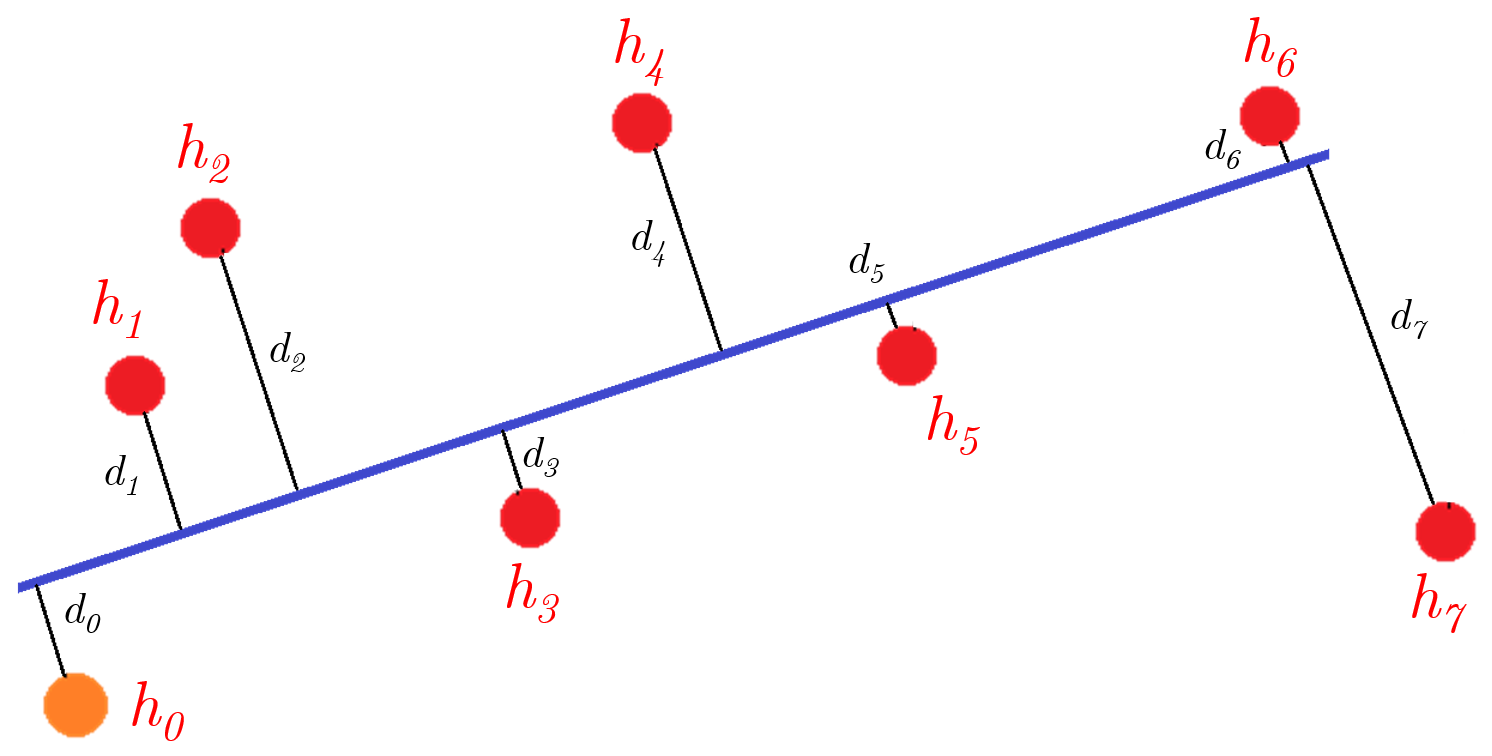
\includegraphics[width=0.9\textwidth]{one_seg.png}
        \caption{One segment, long offshoots}
        \label{fig:one_seg}
    \end{minipage}
    \begin{minipage}{0.45\textwidth}
        \centering
        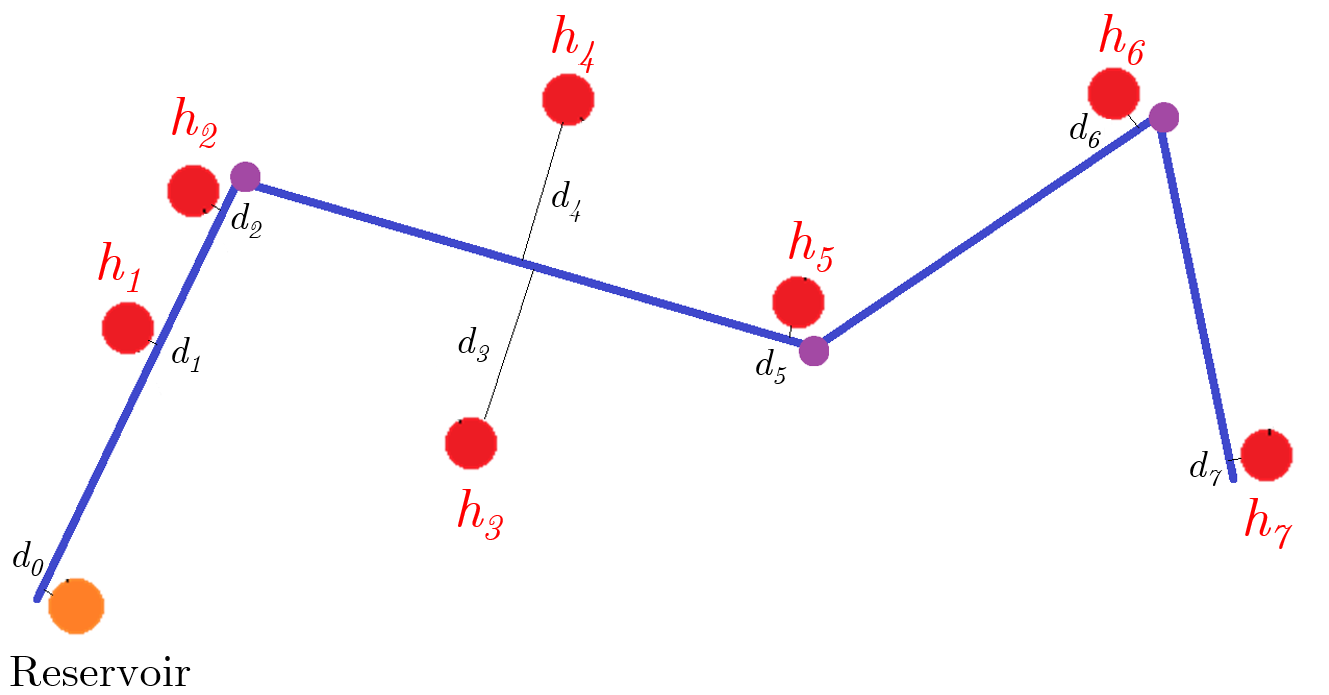
\includegraphics[width=0.9\textwidth]{four_segs.png}
        \caption{Four segments, short offshoots}
        \label{fig:four_segs}
    \end{minipage}
\end{figure}
\vspace{0.1\textheight}
We are now faced with the following problem. The government is only funding the pipe segments (irrespective of their lengths). We need to bear the cost of welding the segments and of the `offshoots' for each house. The cost of welding is $W$ dollars \textbf{per segment}, and the cost of offshoots is $C$ dollars \textbf{per unit length} (remember that \textit{line\_fit} returns the total length of all offshoots). We need to minimize the cost of the project (welding + offshoots). If we have too few segments, we need longer offshoots for the houses, thus driving up the cost. If we have too many segments (e.g. one segment serving each house), you need shorter branches but more welded joints, which can again be costlier. In theory, the number of such arrangements we need to consider is huge (non-polynomial in $n$). We can imagine that there is a certain number of segments that gives us the best trade-off between welding and offshoots, and minimizes the total cost. E.g. figure \ref{fig:two_segs} uses only two segments and the offshoots are not as long as in figure \ref{fig:one_seg}.

\begin{figure}[h!]
    \centering
    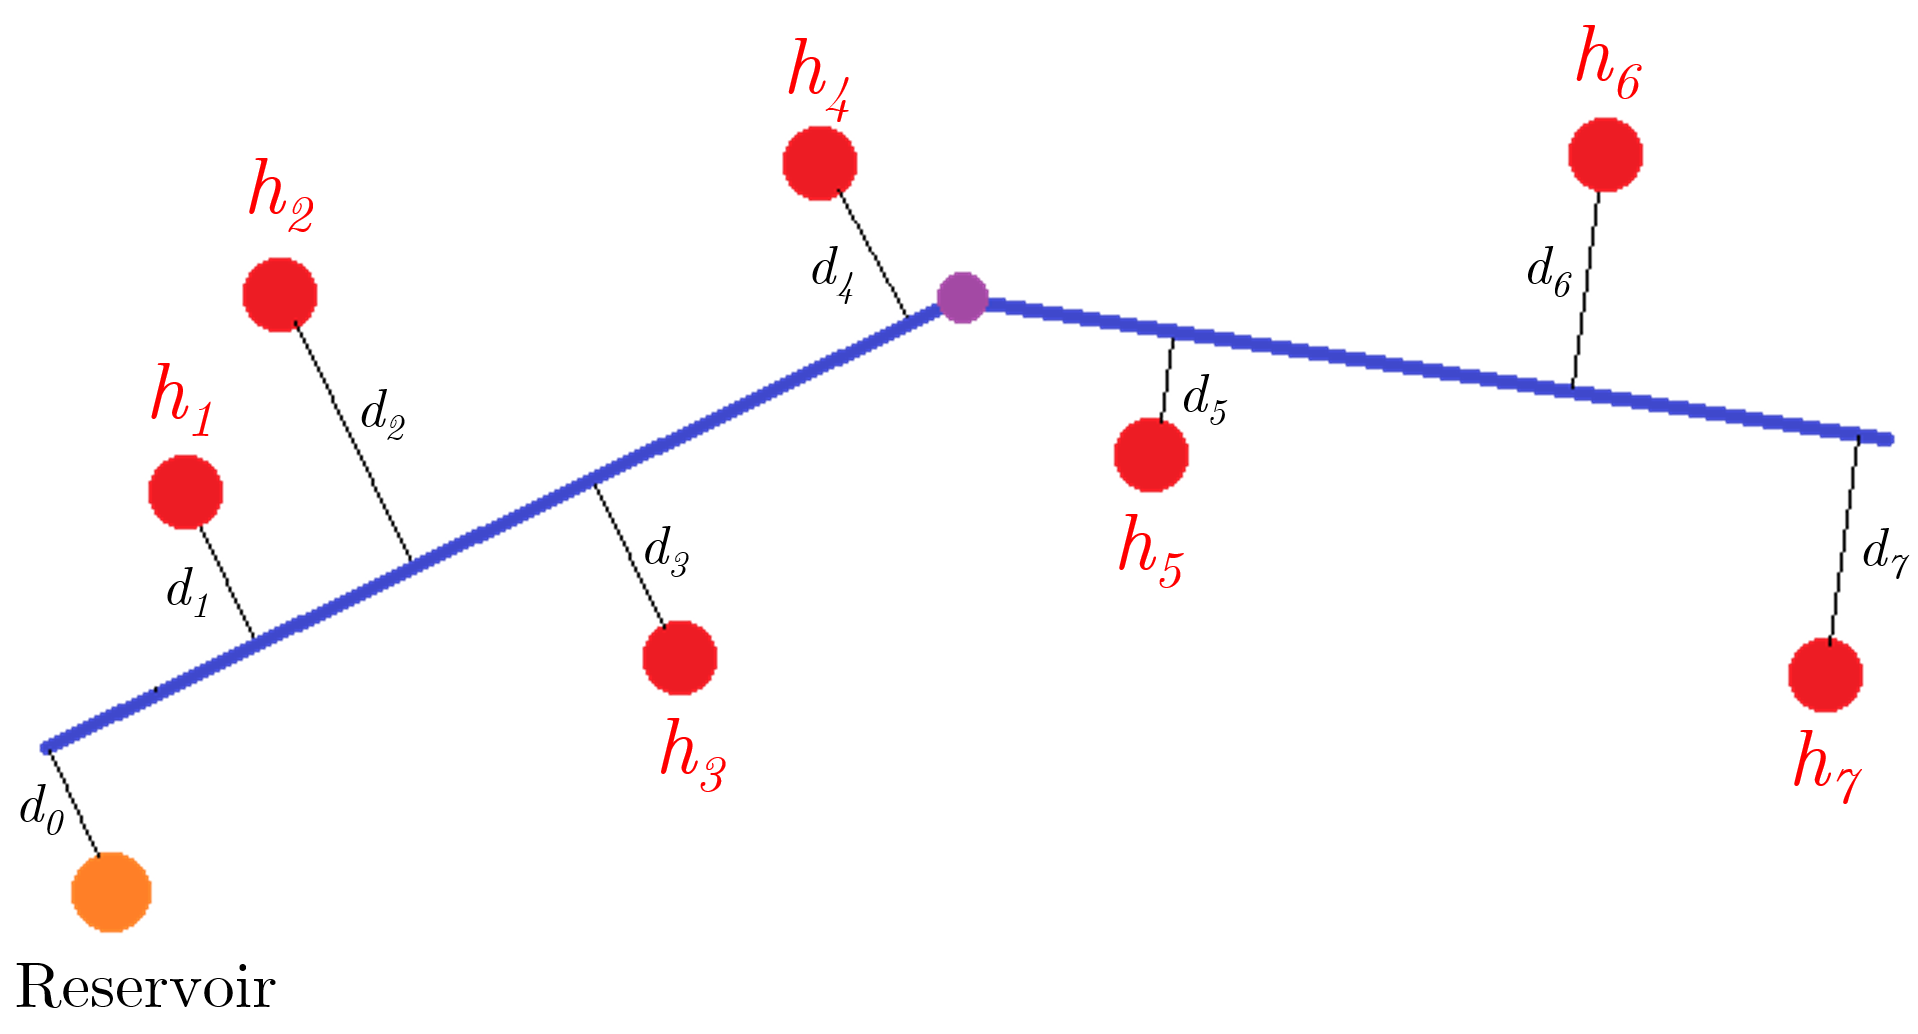
\includegraphics[width=0.4\linewidth]{two_segs.png}
    \caption{Two segments, not too long offshoots}
    \label{fig:two_segs}
\end{figure}

There are certain constraints to be considered. The pipeline has to be one continuous entity without any forks. Each segment must serve only consecutive houses from the given sequence (e.g. a segment cannot serve $h_1, h_2, h_4$ without serving $h_3$). In other words, \textit{line\_fit} only accepts consecutive points $h_i, h_{i+1}, \dots, h_j$ as arguments, and returns the optimal value of $\sum_{r=i}^j d_r$ which is the sum of distances for the line of best fit. Each house must be connected, and every segment of the pipeline must serve at least one house. 

Considering these constraints and using \textit{line\_fit} as a subroutine, answer the following questions.
\begin{parts}
\part[4] Write the cost optimization equation for this problem in terms of $n$, $W$, $C$, and \textit{line\_fit}. [\textit{Hint: The cost of offshoots in each segment is $C$ $\times$ the sum of distances returned by} line\_fit \textit{for that segment. The length of the segment itself does not matter.}]

\mysolution{
\input{Sol-6a}
}

\part[10] Design a dynamic programming algorithm that takes the co-ordinates of the reservoir and $n$ houses as input, and returns the minimum \textbf{cost} of the pipeline.

\mysolution{
\input{Sol-6b}
}

\part[4] Analyze the running time of the algorithm (treat the oracle as constant-time).

\mysolution{
\input{Sol-6c}
}

\part[2] Comment on the benefit of using dynamic programming to solve this problem.

\mysolution{
\input{Sol-6d}
}
\end{parts}

\end{questions}
\end{document}
